\documentclass[main.tex]{subfiles}
% \nomenclature[A]{GPR}{Ground Penetrating Radar}%

\begin{document}
\chapter{Concept Design}
\chaplabel{conceptDesign}

This chapter presents the design requirements and concept solutions for the various project subsystems, namely the sensor subsystem, including signal processing and sensor fusion, the platform subsystem, including automation and navigation, and the sensor mount subsystem.

\section{Sensor selection}
The selection of sensors for the project was based on the requirements from the scenario of operation. These are as follows:

\begin{itemize}
\item The sensor suite should be able to detect anti-personnel and anti-tank mines with high and low metal content 
\item Real time detection at an operational speed of 5 km/h and depths of up to 15 cm
\item The chosen sensors must be able to discriminate between landmines and other objects, with an aim to minimise false positives
\end{itemize}

As outlined in the benchmarking section, the primary sensors used for landmine detection operations are metal detectors and GPRs. When used in isolation, each sensor has several limitations. Metal detectors can only be used to detect metallic mines, they produce a large number of false positives, and their penetration depth is restricted. On the other hand, GPR systems produce data that is difficult to interpret, and is also very sensitive to environmental conditions such as soil type and moisture content. In both cases, signal processing of some form is required, either using software to identify detected objects, or with the involvement of a skilled operator.

Multisensor systems allow a greater range of targets to be identified. In addition, having two sensors provides the ability to confirm the presence of metallic mines, which reduces false positives and thereby increases the efficiency of operations. While it is difficult to quantify this increase in efficiency, this result has been demonstrated in experimental work carried out by \textcite{Takahashi10}. As can be seen in \Figref{FAR}, the false alarm rate, defined as the number of false alarms per unit area, for a system that combines a metal detector and GPR is roughly half that of a metal detector alone. Thus, a multisensor system meets the necessary requirements outlined above, while addressing some limitations of individual sensor systems.

\begin{figure}[ht]
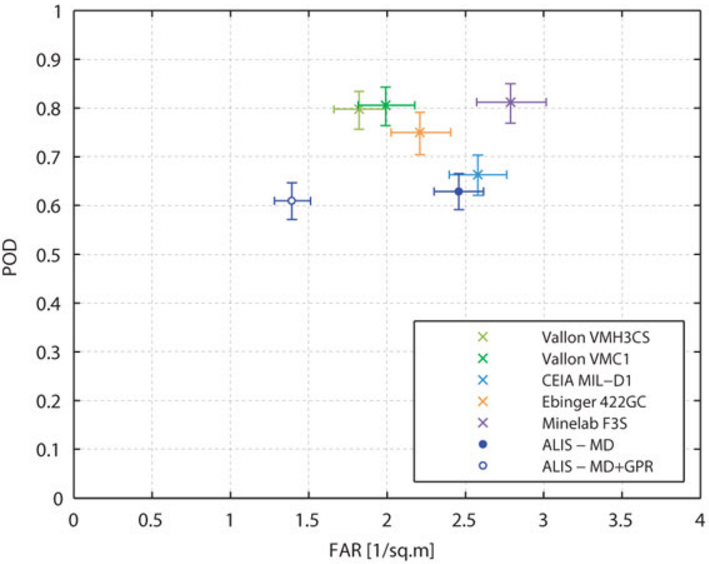
\includegraphics[width=0.6\textwidth]{3-ConceptDesign/FAR.PNG}
\centering
\caption[Reduction in false alarm rate observed as a result of using a multisensor system]{Reduction in false alarm rate observed as a result of using a multisensor system (ALIS-MD+GPR) as opposed to a metal detector alone \parencite{Takahashi10}} \figlabel{FAR}
\end{figure}

Initially, it was expected that the sensor suite would be comprised of a metal detector array and a GPR array provided by the DSTG, with a total payload weight of 80 kg. The use of the 3 m wide arrays would allow for larger areas to be scanned in a shorter period of time, leading to an increase in operational efficiency. Due to unforeseen circumstances, the arrays could not be made available for the project, and so smaller line scan sensors had to be used instead. Off-the-shelf sensors were then considered, however most were not able to produce any raw data output that could be processed to meet the project objectives. In the case of GPR systems, the high cost of systems was also a limiting factor. Eventually, a pair of sensors were borrowed from the DSTG, the specifications of which are presented below. Despite the fact that line scan sensors were used, it was assumed that the scanning arrays would be made available by the completion of the project, and so the size and weight specifications of the arrays were used in selecting the platform and designing the sensor suite. 

\subsection{AMDS metal detector panel}
The AMDS is a metal detector panel produced by Minelab (\Figref{AMDS}). The device has three sets of transmitting coils and a single receiving coil, allowing for three channels of data to be recorded at once. Each channel operates at four frequencies, 1.5 kHz, 4.5 kHz, 13.5 kHz and 40.5 kHz, which means that in total up to 12 sets of data can be recorded simultaneously. This recorded data contains the real and imaginary parts of the voltage signal measured due to changes in magnetic flux in the target. The data is transferred to a computer through USB, where it can be seen in real-time using a LabVIEW virtual instrument called Dataspleen, or saved in CSV format. The metal detector requires a 10 volt power supply at 0.5 amps.  

\begin{figure}[ht]
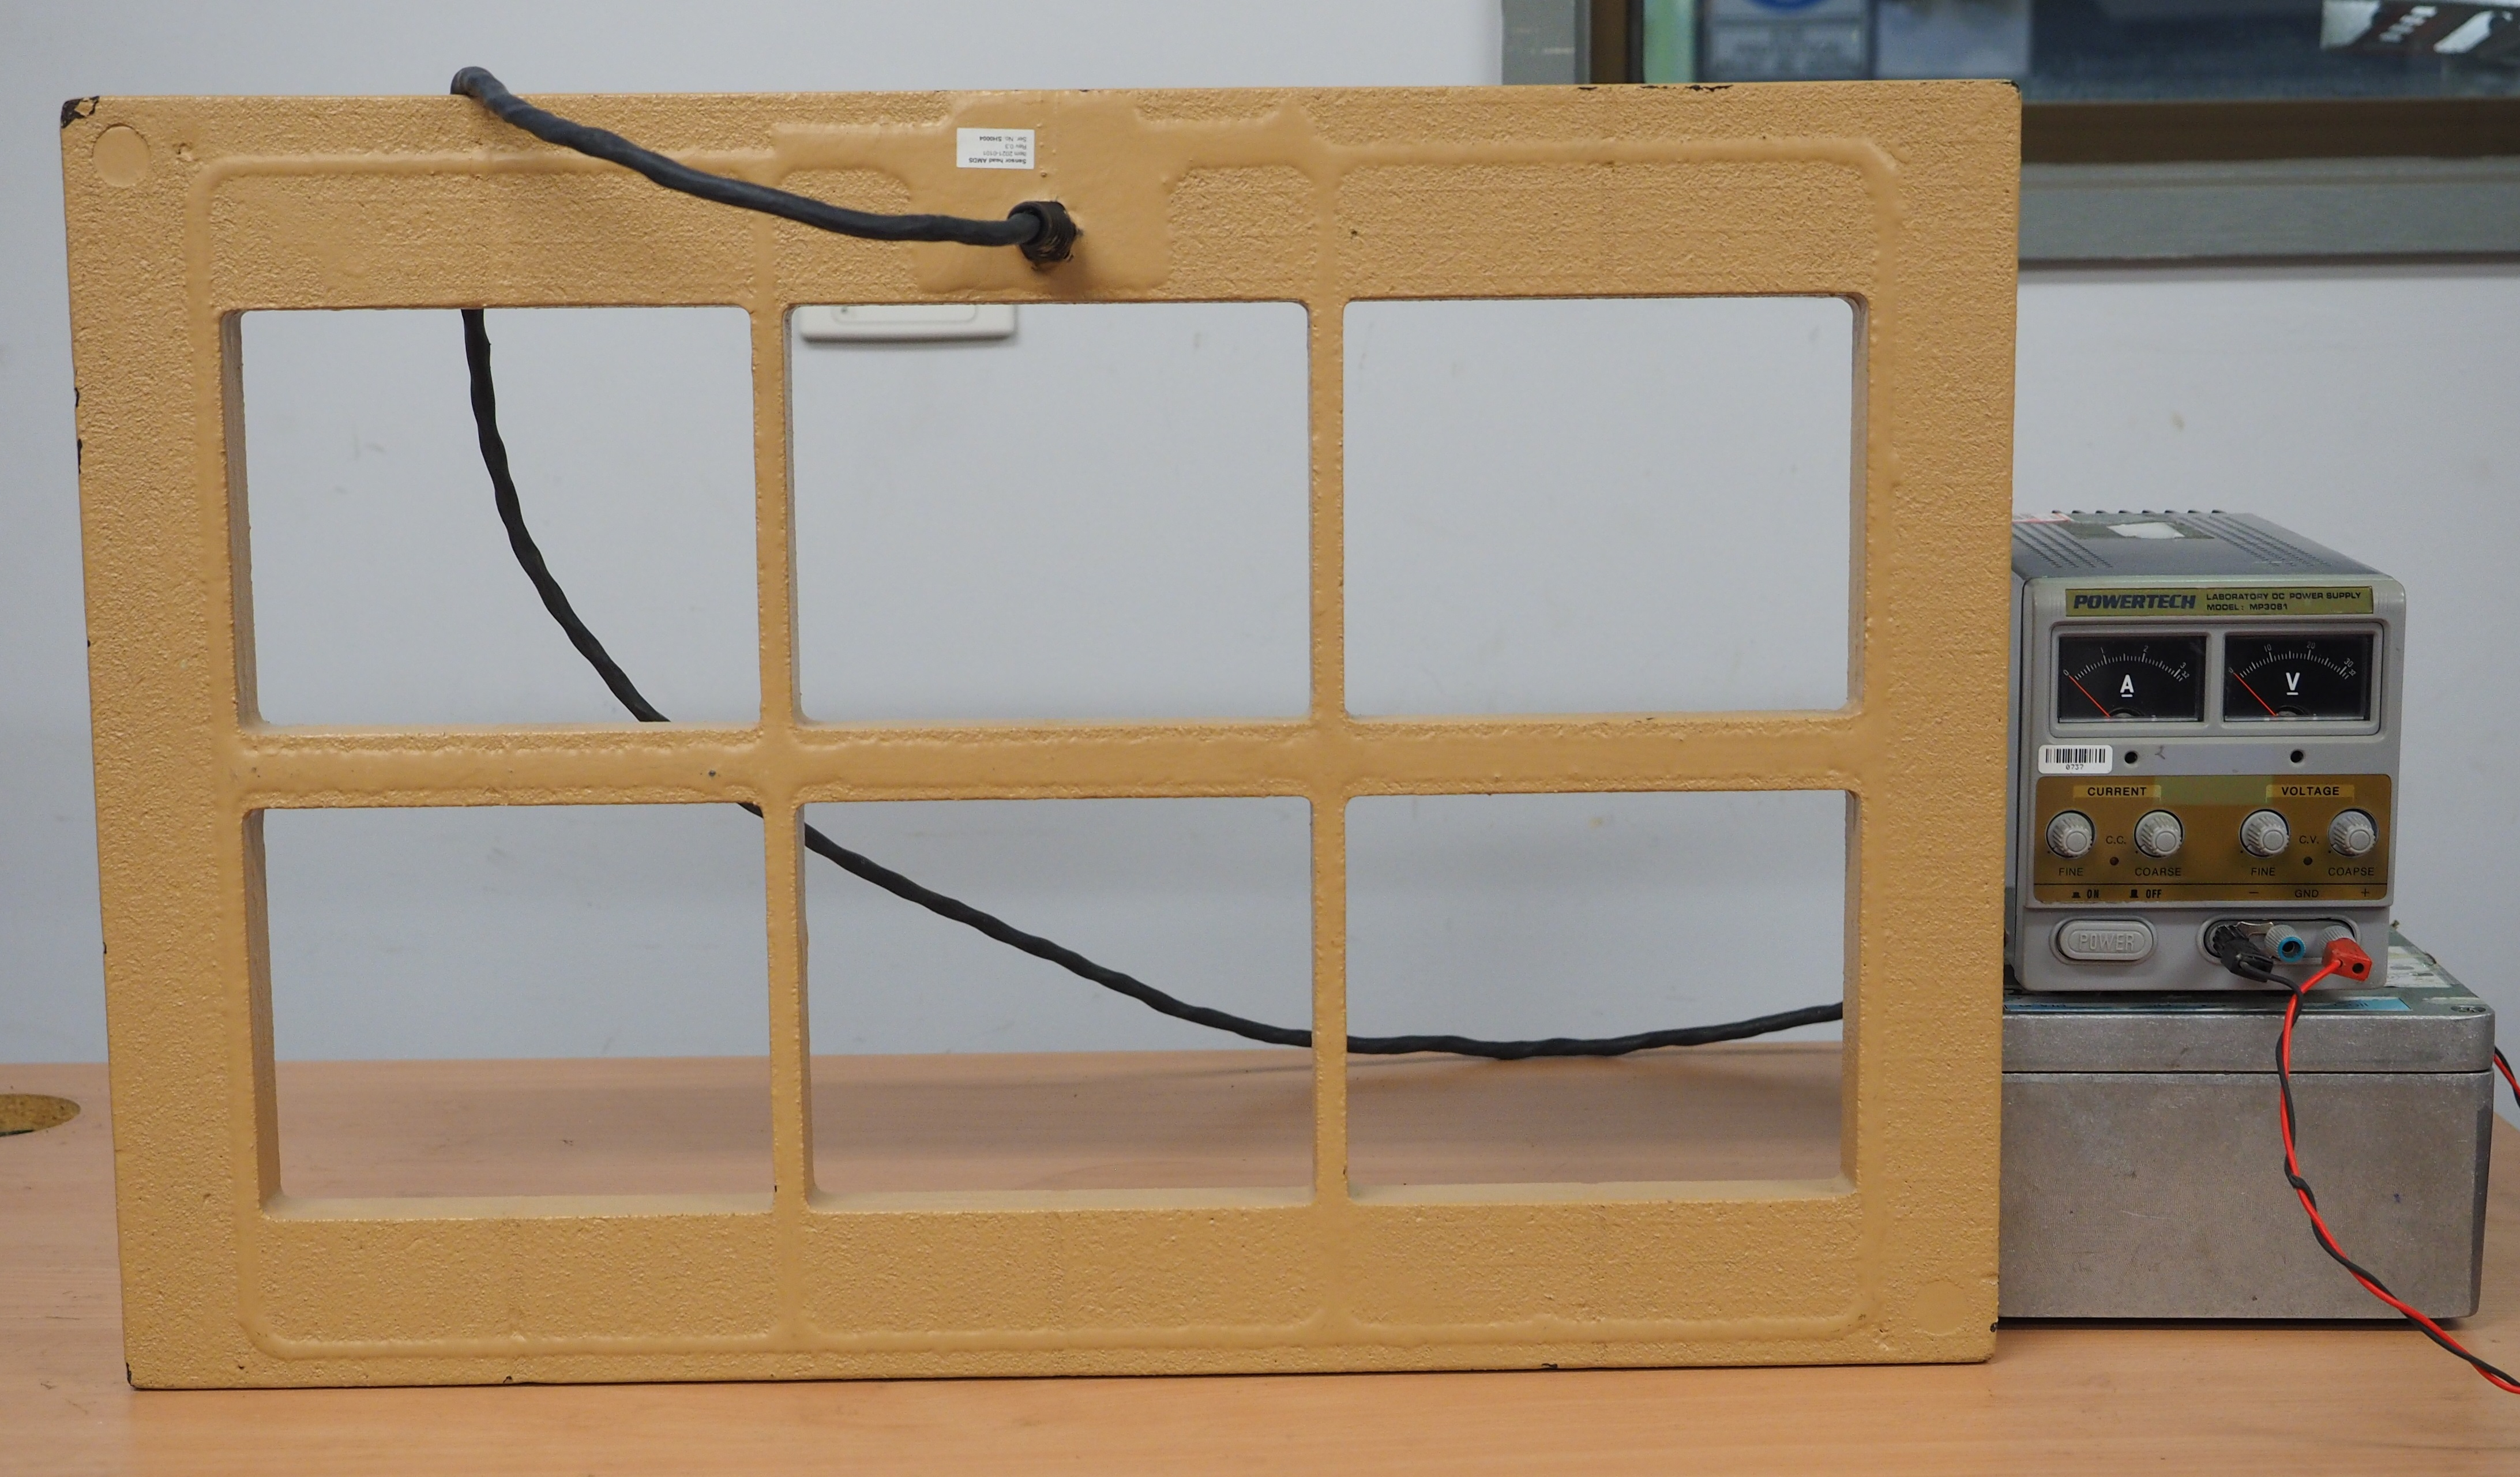
\includegraphics[width=0.5\textwidth]{3-ConceptDesign/AMDS.JPG}
\centering
\caption{AMDS metal detector panel with power supply and control unit} \figlabel{AMDS}
\end{figure}

\subsection{SIRO-PULSE II GPR unit}
The SIRO-PULSE II is a handheld GPR unit developed by the CSIRO, originally intended for the inspection of buildings (\Figref{siro}). It is a pulsed radar that can operate in either bi-static or differential antenna configurations, producing three sets of data in total. The unit comes with three interchangeable antenna heads of frequencies 800 MHz, 1.4 GHz and 2 GHz, allowing the resolution and penetration characteristics of the radar to be varied. Data is transferred to a computer via USB, where it can be viewed in real-time with the accompanying SiroPuleII software program. The program produces outputs of the frequency waveform over time, which are collected together to produce a B-scan in real time. The unit is battery powered with a runtime of up to 10 hours. 

\begin{figure}[ht]
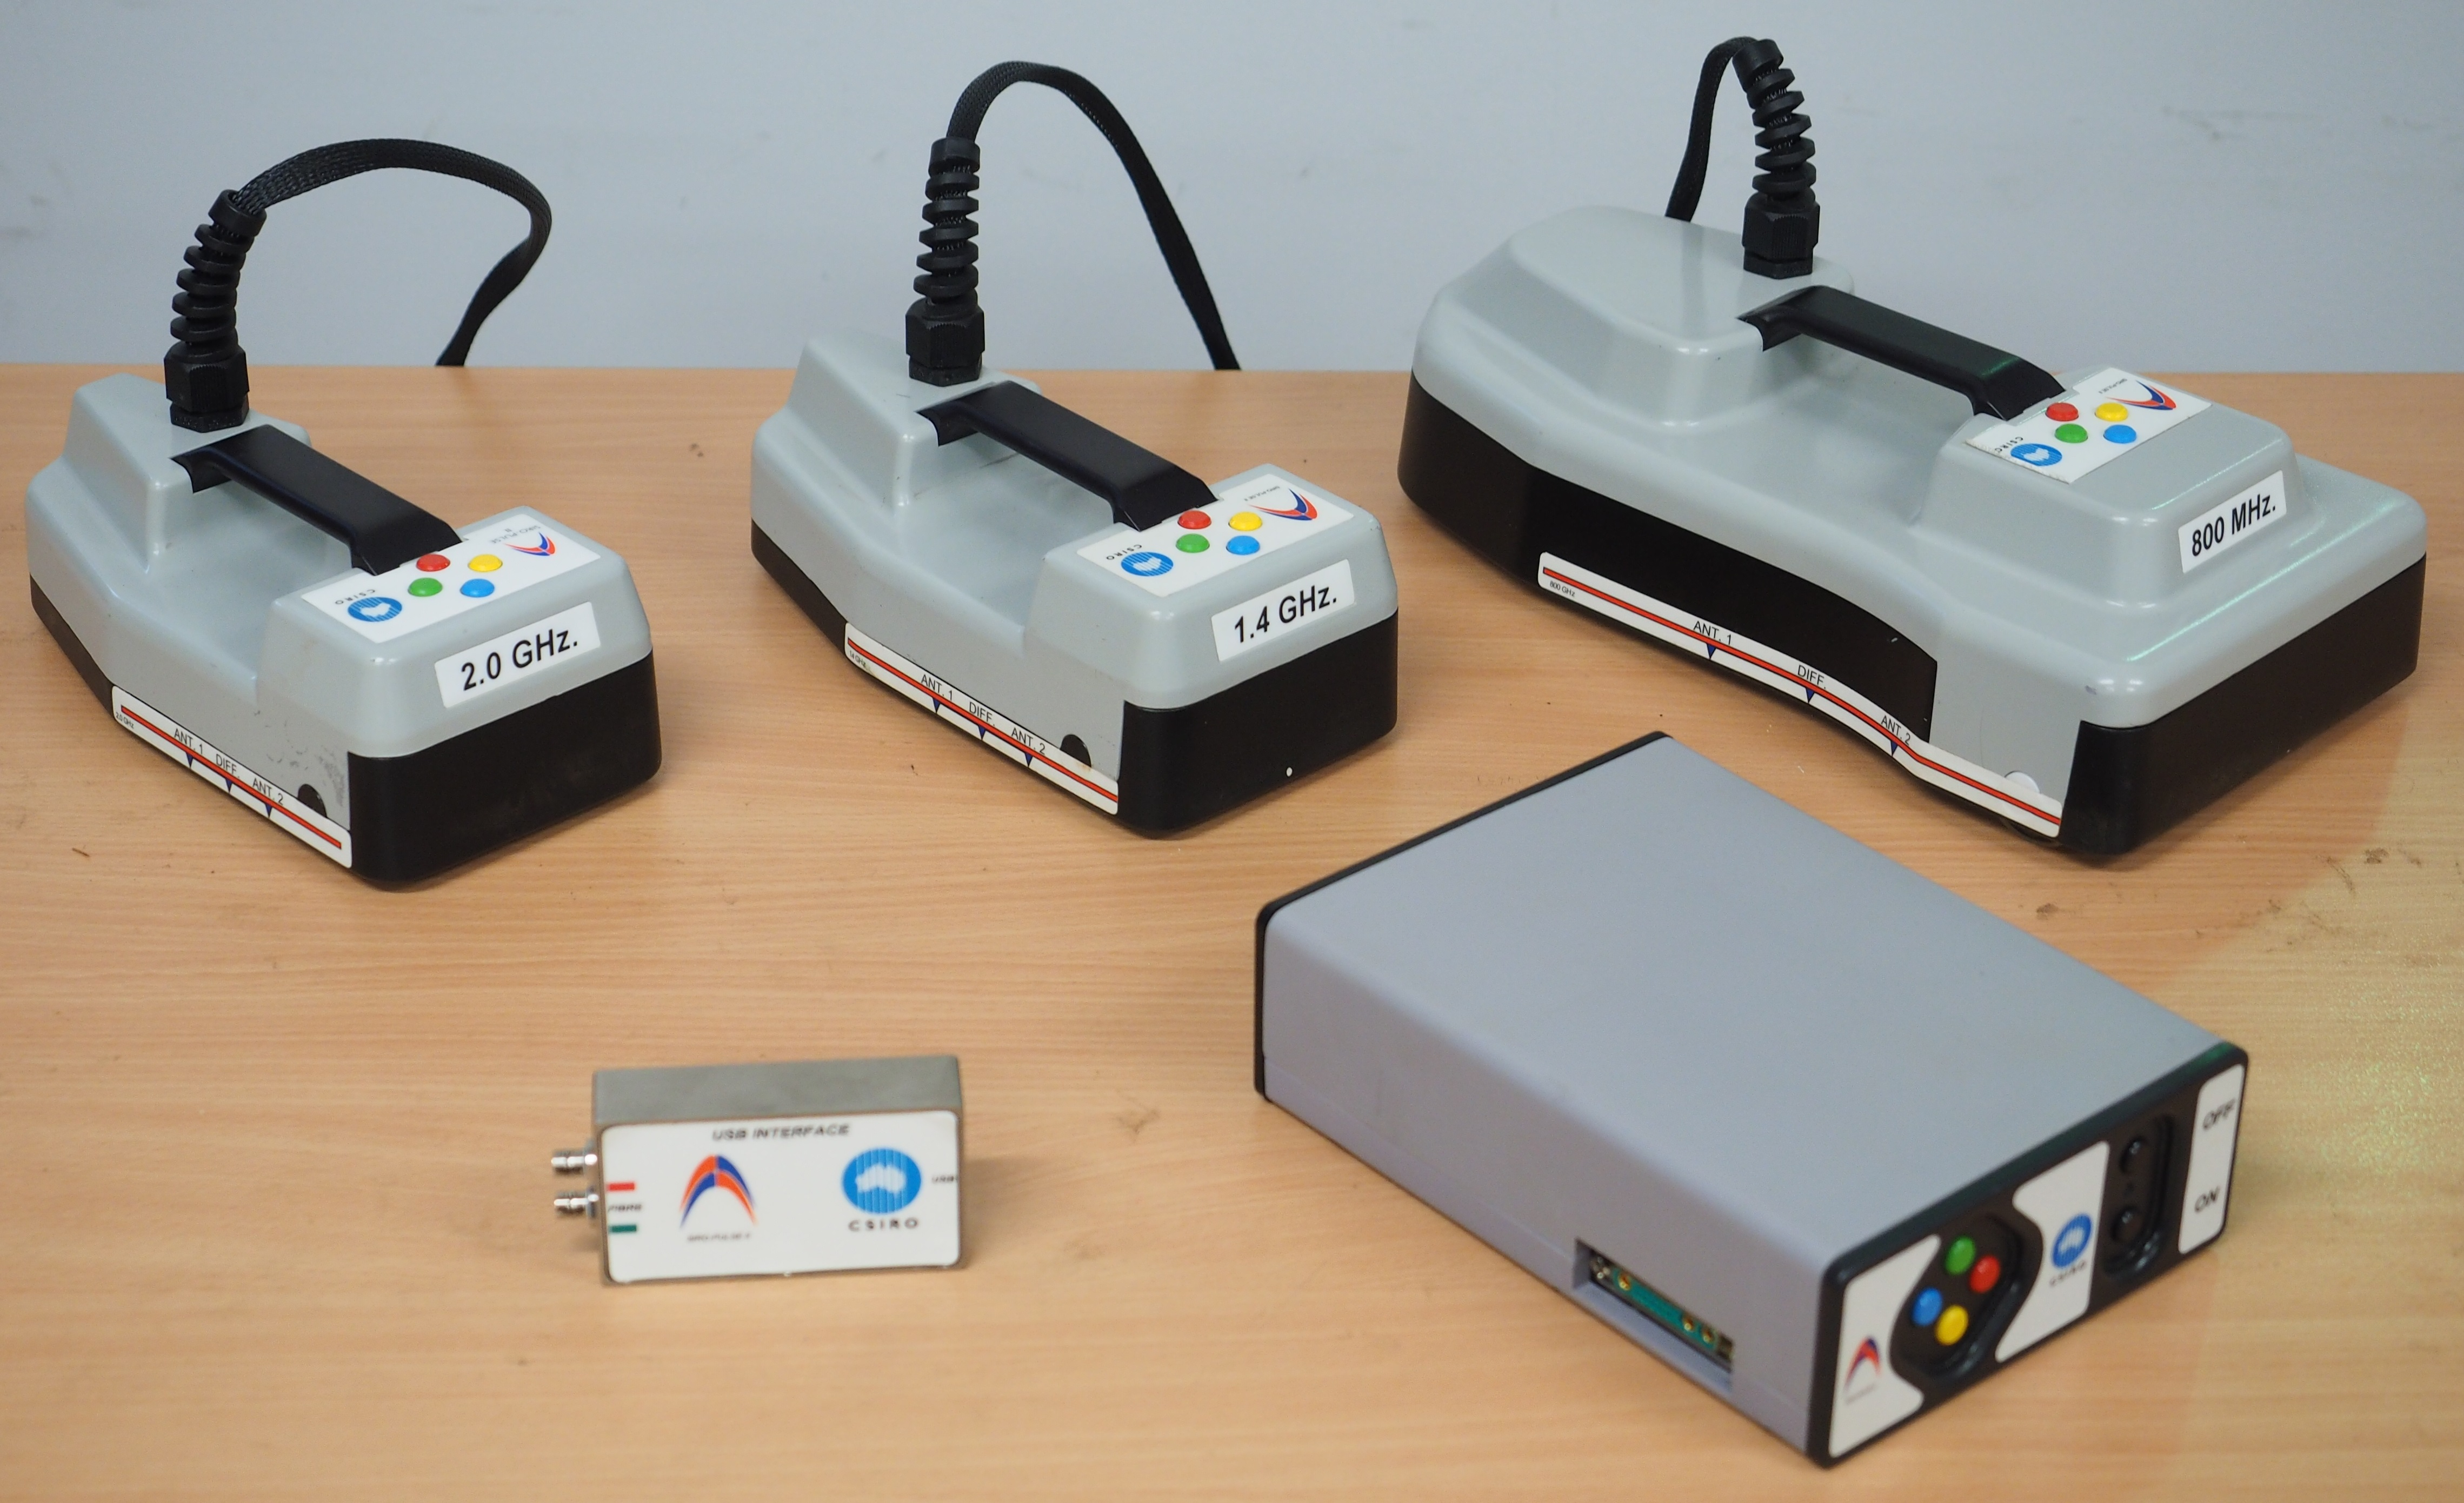
\includegraphics[width=0.5\textwidth]{3-ConceptDesign/SiroPulse.JPG}
\centering
\caption{SIRO-PULSE II GPR unit with control unit and antenna heads} \figlabel{siro}
\end{figure}

\section{Sensor fusion and signal processing}
Regardless of the fact that the sensors suite met the outlined requirements, there were several key challenges to be addressed, namely sensor fusion and signal processing. The first of these relates to how the data from the separate sensors can be consolidated to provide a single meaningful result, while the second involves processing the output from the sensors to allow an operator to identify targets. 

\subsection{Sensor fusion}
As discussed in the literature review, there are three primary levels of sensor fusion, decision level, feature level and data level \parencite{Yarovoy2009}. Of these, decision level sensor fusion was selected as it offers the simplest and least computationally intensive solution, since the outputs from the sensors can be processed individually. This method also lends itself well to machine learning techniques, allowing a target to be identified based on correlations with a known dataset. The main disadvantage of this method is that it is not as robust as the other methods, however this was not expected to be an issue given the scope of the project. 

To be able to implement decision level sensor fusion, a decision needs to be made with each sensor regarding whether or not the target is a mine. This decision, along with a confidence interval, can be passed onto the sensor fusion algorithm as shown in \Figref{fusion}, which assigns then makes the final decision based on a weighted evaluation of the data it has received. In order for each sensor to make a decision, metrics need to be identified which can be used to characterise targets. As a result, preliminary tests were carried with both sets of sensors to find such metrics.

\begin{figure}[ht]
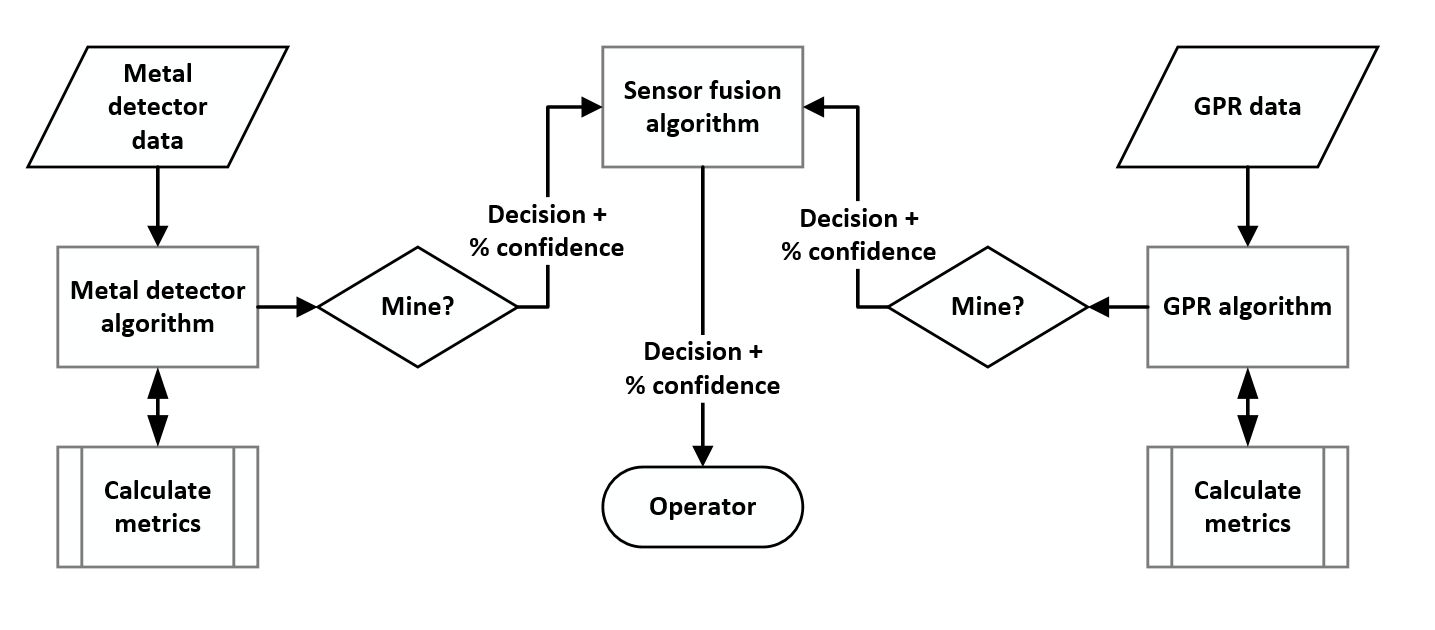
\includegraphics[width=0.85\textwidth]{3-ConceptDesign/fusion.PNG}
\centering
\caption{Integration of signal processing and sensor fusion algorithms} \figlabel{fusion}
\end{figure}

\subsection{Metal detector output}
Initial tests with the metal detector were performed indoors. In the first set of tests, horizontal sweeps were made over a number of small metal samples (\Figref{samples}) placed on the floor, with the distance to the metal detector being kept constant at 32 cm. 

\begin{figure}[ht]
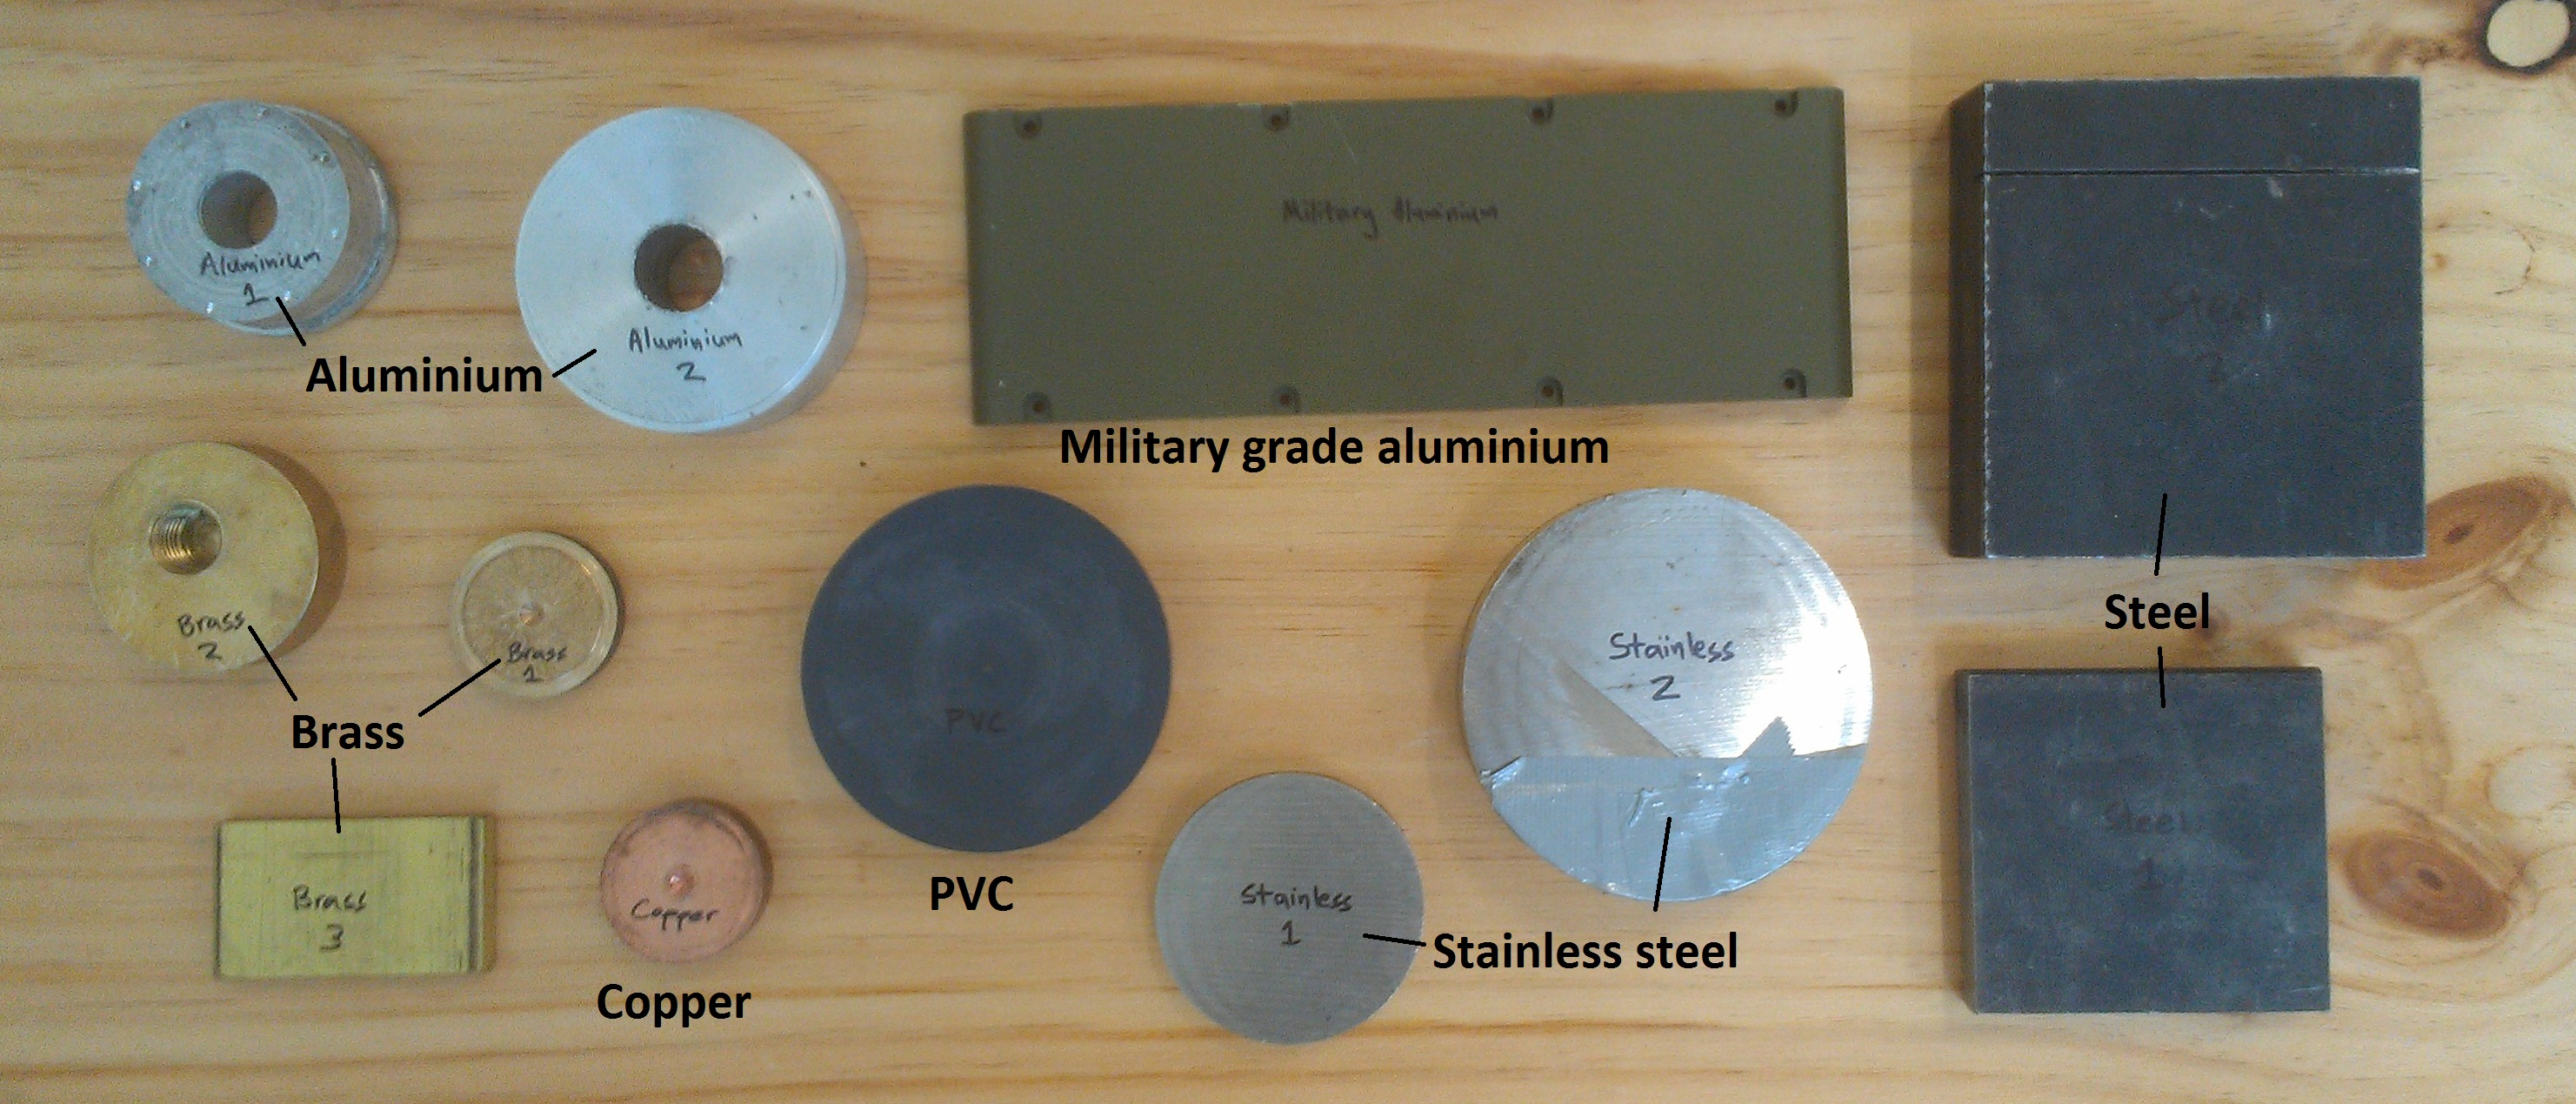
\includegraphics[width=0.8\textwidth]{3-ConceptDesign/samples.jpg}
\centering
\caption{Metal samples used for evaluation of metal detector outputs} \figlabel{samples}
\end{figure}

\Figref{metals} shows the results obtained from the second channel plotted in Matlab. The four lines in each plot correspond to the four frequency signals, while the axes represent the real and imaginary components of the voltage signal. It can be seen that for different metals, the magnitude and phase angle of the signal vary, as discussed in the literature review. 

\begin{figure}[ht]
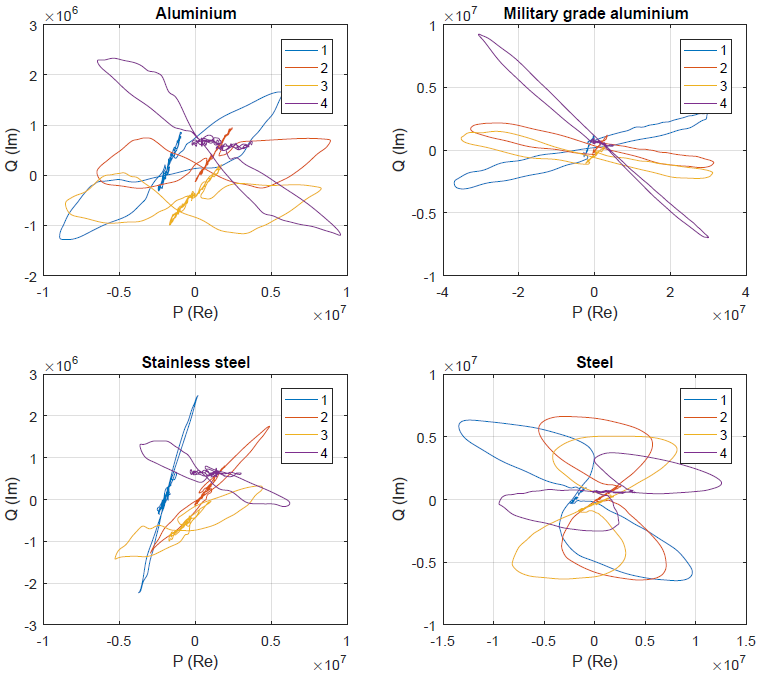
\includegraphics[width=0.65\textwidth]{3-ConceptDesign/metals.PNG}
\centering
\caption{Phase plots for several different metal samples at 32 cm depth} \figlabel{metals}
\end{figure}

In the second set of tests, a single brass sample was scanned, with the distance to the metal detector changed between scans. The results are shown in \Figref{phaseDepth}, and while the phase angle does not vary with depth, the signal magnitude does. Based on on these tests, it was concluded that the magnitude and phase angle of the signal would be suitable metrics for characterising objects; the phase angle can be used to identify the metal, while the magnitude provides information about the depth, size and material. Thus, the aim of the signal processing algorithm for the metal detector is to find these metrics given the metal detector input data. 

\begin{figure}[ht]
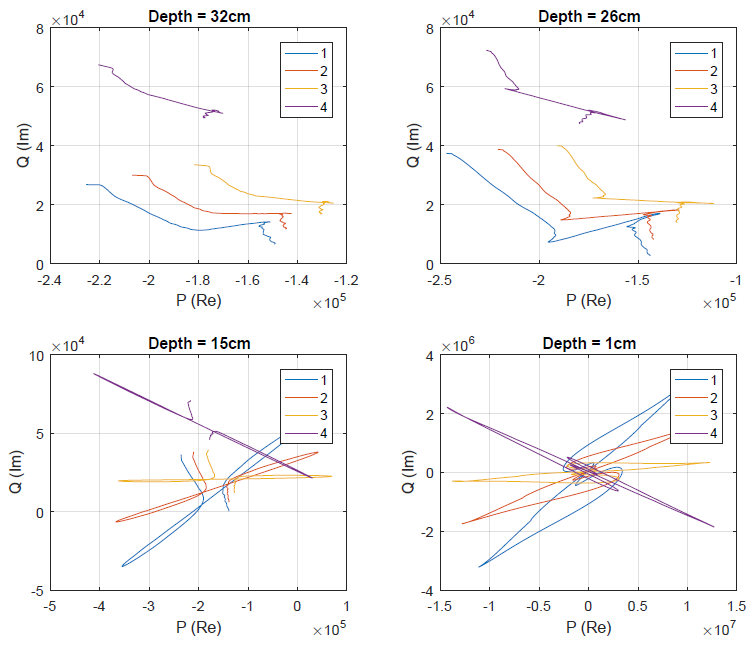
\includegraphics[width=0.65\textwidth]{3-ConceptDesign/phaseDepth.PNG}
\centering
\caption{Phase plots for a brass sample scanned at different depths} \figlabel{phaseDepth}
\end{figure}

\subsection{GPR output}
Preliminary tests for the GPR could not be conducted at the same time as metal detector testing due to issues in operating the GPR. However, sample datasets were provided by the DSTG, and these were analysed in Matlab. \Figref{cans} shows the B-scans for an empty (background) scan, as well as a scan over two soft drink cans. 

Unlike with the phase plots obtained from the metal detector, it was not as clear what metrics could be identified from the GPR data. To further aid in visualising the signal, the background was subtracted (\Figref{cansNoBG}). This made it easier to identify features in the scan, the size and position of which could be found easily. Once the position of the feature is known, the A-scan corresponding to the feature can be extracted, and this can also be used to characterise the feature. Hence, the chosen metrics for the GPR are feature size, feature position and A-scan characteristics.

\begin{figure}[ht]
\centerline{
\begin{tabular}{cc}
\subfloat[]{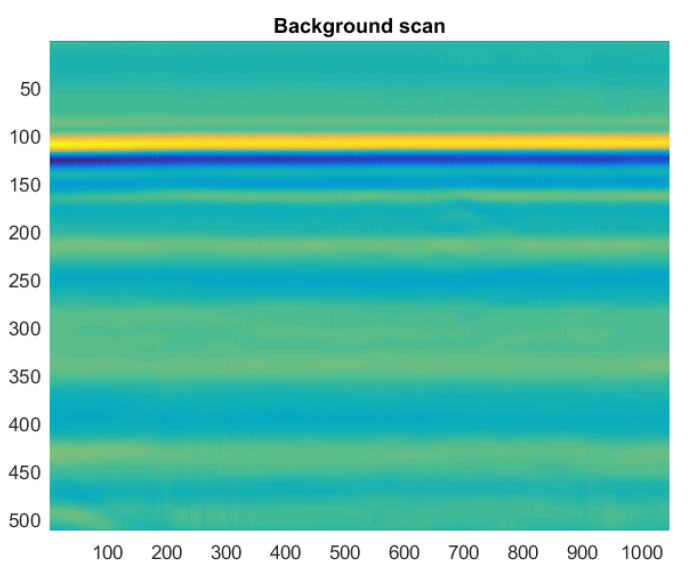
\includegraphics[width=0.46\textwidth]{3-ConceptDesign/bg.PNG}}
& \subfloat[]{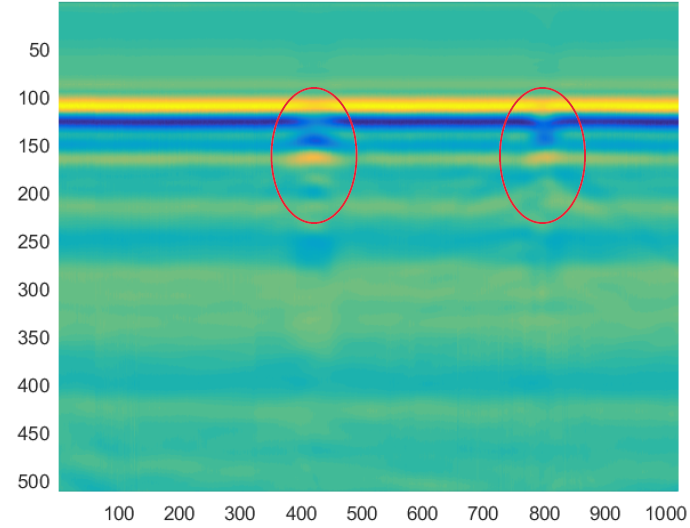
\includegraphics[width=0.46\textwidth]{3-ConceptDesign/cans.PNG}}\\
\end{tabular}}
\caption{Background scan (a) and B-scan over two soft drink cans, circled in red (b)} 
\figlabel{cans}
\end{figure}

\begin{figure}[!ht]
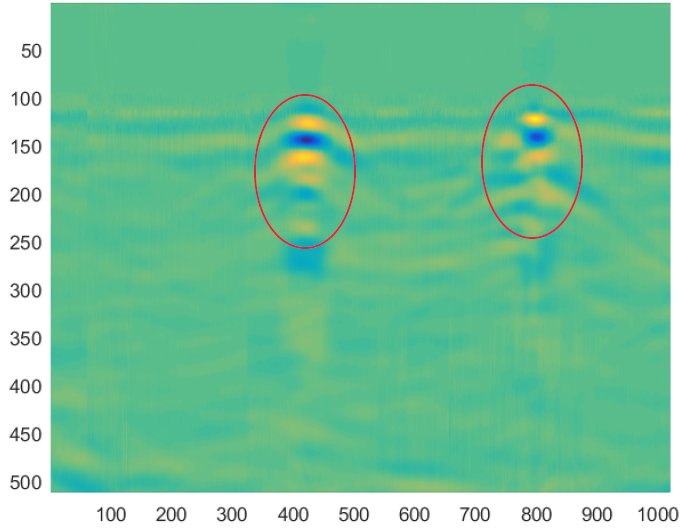
\includegraphics[width=0.6\textwidth]{3-ConceptDesign/cansNoBG.PNG}
\centering
\caption{B-scan for soft drink cans with background removed} \figlabel{cansNoBG}
\end{figure}

\section{Platform selection}
\seclabel{platformselect}
A detailed platform selection process was carried out, as outlined in \Chapref{platformSelectionApp}. 

The platform is used to mount the required detection equipment and acts as the foundation for a completely autonomous system. The design and construction of a new platform was considered to be outside the scope of the project, and so the modification of an existing platform was the preferred approach. The requirements for the platform primarily come from the scenario of operation, but also include considerations such as budget and availability. as well as the budget

\begin{itemize}
 \item Carry a total payload of 100 kg. A pair of metal detector and GPR arrays with their respective control boxes have an estimated gross weight of 80 kg. This allows 20 kg for any mounting structures,  electronics and computers. 
 \item Travel off-road in regions with dry sandy soils and level unobstructed terrain.
\item Travel in a straight line, both forwards and reverse, and perform turns while maintaining an operational speed of 5 km/h.
\item Be manoeuvrable enough to navigate the region of interest, yet controllable enough than in case of an emergency, it can come to a complete stop from its operational speed in 1 m.
\item Availability to the project
\item Cost: Based on a budget of \$16,500. A platform cost nearing \$5,000 indicated that the requirement had been met. A score of 10 indicates platform supplied in-kind and 1 indicates financially infeasible.
\item Portability: Level of portability. A higher score indicates simpler transport with less disassembly required. The requirement had been satisfied if transport was possible in the back of a ute or trailer.
\item Implementation of Auto-Control: How involved the process of implementing the direct hardware required for remote operation would be. A low score indicates a difficult process with many sub-systems, whereas a high score indicates little to no work necessary. Requirement was met if implementation of hardware was a feasible task.
\item Control/Manoeuvrability: How appropriate the platform was expected to be regarding manoeuvrability assuming auto-control was implemented successfully. This included speed, acceleration, turn radius, and stopping distance.
\item Implementation of detection equipment: Ease of installation of detection equipment and expected effectiveness of the platform and sensor combination from a landmine detection point of view.
\end{itemize}

%\subsection{Utility Quad Bike}
Quad bikes are designed as all terrain vehicles and are capable of traversing even the most demanding terrains. Utility quad bikes are intended to carry large loads as well as a human operator and so load limits are frequently larger than 100 kg. Due to the nature of the platform and through visual inspection, mounting points for sensor brackets and electronic systems are located in various positions.  Environmental conditions are of little concern to this platform which will be encountered and traversed with ease for ranges of over 100 km. Turning radius for quad bikes are typically in the range of 3-4 metres.
The DSTG have offered the use of one of their autonomous quad bikes to be used as the platform. The DSTG quad bike is a Honda TRX450r and has a weight load capacity of 110 kg. The quad bike has been previously fitted with remote control capabilities and is in good working condition, however \textcite{scheiner2011} recommended that the brake actuator be replaced as well as some electronics. As the platform already has remote control capabilities, transport becomes a much easier task especially with a trailer or ute with a ramp.
\begin{figure}[ht]
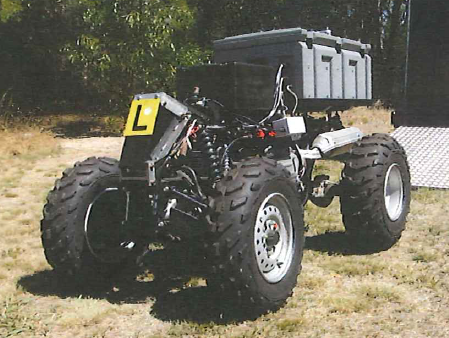
\includegraphics[width=0.4\textwidth]{3-ConceptDesign/2011quadbike.PNG}
\centering
\caption[DSTG autonomous quad bike]{DSTG autonomous quad bike \parencite{scheiner2011}} \figlabel{2011quadbike}
\end{figure}

%\subsection{Dune Buggy}
A dune buggy is a vehicle designed for high speed operation on loose, sandy terrain. Design of dune buggies are commonly an open chassis housing a modified vehicle and thus it's performance characteristics are similar or better than that of a small car. They are commonly able to carry two persons resulting in a load capacity exceeding 160 kg. Dune buggies frequently have turn radii around 6 metres restricting path curvature for accurate tracking. Due to the nature of the platform equipment mounting is common practice and would not raise any issues however a bare mass of 230 kg and dimensions 2.3 by 1.5 metres would make the unit difficult to transport.
\begin{figure}[ht]
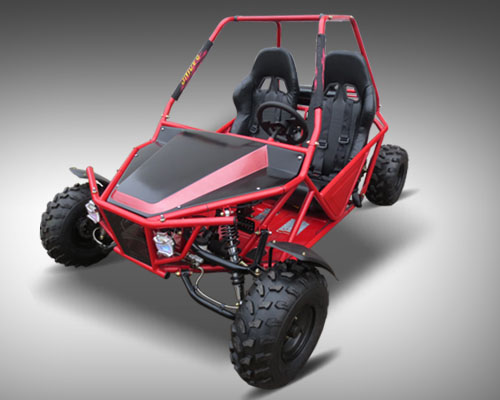
\includegraphics[width=0.4\textwidth]{3-ConceptDesign/kandidunebuggy.jpg}
\centering
\caption[Kandi-150 dune buggy]{Kandi-150 dune buggy \parencite{150GKM}} \figlabel{kandi150}
\end{figure}

%\subsection{Continuous Track Vehicle}
Tracked vehicles are designed to distribute the weight of the vehicle over a large area enabling the traversing of soft and loose terrain without the concern of losing traction and becoming stuck. The platform shown in \Figref{grillon500} is one example of such a vehicle. The Grillon-500 is able to carry a payload of 1000 kg and operate at speeds up to 11 km/hr however a bare mass of 100 kg and dimensions of 1.5 m by 2.5 m could make the unit difficult to transport \parencite{cinamGrillon}. This model is designed to support the mounting of various equipment in the front bay (fork lift pictured). An advantage of the tracked vehicle over other platforms is its ability to turn on the spot eliminating the need for complicated turn algorithms. 
\begin{figure}[ht]
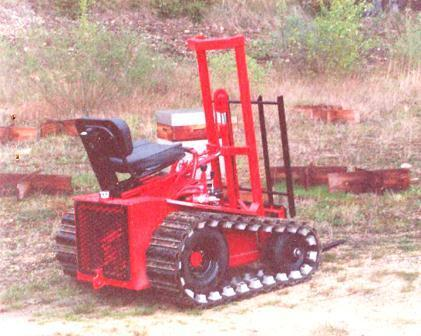
\includegraphics[width=0.4\textwidth]{3-ConceptDesign/Grillon-500.jpg}
\centering
\caption[Grillon-500 tracked vehicle]{Grillon-500 tracked vehicle \parencite{cinamGrillon}} \figlabel{grillon500}
\end{figure}

%\subsection{Hovercraft}
Access was made available to an existing hovercraft from a 2009 University of Adelaide Honours Project. Analysis of the technical report \parencite{hovercraft2009} and practical and theoretical evaluations showed that the lift fan was able to support a payload of up to 22 kg and the thrust fans were only just capable of moving the craft on a flat, smooth surface. For complete automation only actuators for the lift motor would be required as remote operation for the thrust system had already been implemented. The stopping distance is lacking due to the time required to rotate fans for reverse thrust. The hovercraft has an advantage over other platforms through its ability to pass directly over a landmine without detonation occurring, however, this 'sliding' advantage introduces new problems when developing a path tracking algorithm due to the advanced dynamics of the platform. The purchasing of a recreational hovercraft more suited to the requirements would not have been financially feasible. Through verbal discussion with DSTG, it was revealed that vibrations produced through the lift and thrust systems on hovercraft platforms were detrimental to the effectiveness of the sensor equipment. Thus, the DSTG has advised against the use of a hovercraft as the platform for landmine-detecting purposes.
\begin{figure}[ht]
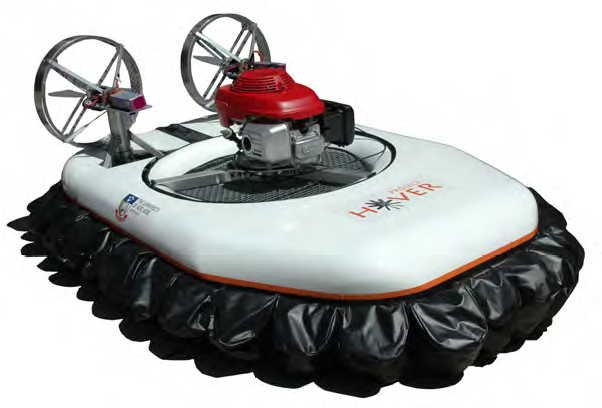
\includegraphics[width=0.4\textwidth]{3-ConceptDesign/HovercraftPic.png}
\centering
\caption[University of Adelaide 2009 Honours Project hovercraft]{University of Adelaide 2009 Honours Project hovercraft \parencite{hovercraft2009}} \figlabel{hovercraftPic}
\end{figure}

%\subsection{Platform Decision}
\Tabref{platformDecision} summarises the strengths of each of the considered platforms. A score of 5 indicated that a requirement had been satisfied or that the criterion was only just feasible for that platform, with any difference being representative of a rise or fall in the platforms specified capability. Scores had a lower limit of 1 and an upper limit of 10. It was evident that the hovercraft did not meet majority of the requirements to be the supporting platform. Commercial quad bikes or dune buggies could have been used with some modifications to the structure, however a tracked vehicle or the quad bike offered by DSTG were clearly the two best options.

The DSTG quad bike was selected over a tracked vehicle for a number of reasons. These included direct availability, financial restrictions, and the completed state of auto control hardware already on the quad bike.
\begin{table}[ht]
\centering
\caption{Platform decision matrix}
\tablabel{platformDecision}
\begin{tabular}{r *6c}
    \multicolumn{1}{r}{}  & \mcrot{1}{l}{45}{Hovercraft (2009)} & \mcrot{1}{l}{45}{Commercial Quad Bike} & \mcrot{1}{l}{45}{Dune Buggy} & \mcrot{1}{l}{45}{Tracked Vehicle} & \mcrot{1}{l}{45}{Quad Bike (DSTG)}\\ \toprule 
    Unit Cost & 10 & 5 & 3 & 4 & 10\\ 
    Implementation of Auto Control & 5 & 3 & 3 & 5 & 9\\ 
    Control/Manoeuvrability & 3 & 7 & 5 & 9 & 7\\ 
    Implementation of Detection Equipment & 1 & 6 & 6 & 5 & 6\\ 
    Payload & 2 & 8 & 10 & 7 & 7\\ 
    Terrain Traversibility & 3 & 9 & 7 & 10 & 9\\ 
    Portability & 7 & 6 & 4 & 8 & 6\\ 
    Navigation & 9 & 5 & 4 & 7 & 5\\ \midrule
    \textbf{Total} & 48\% & 64\% & 57\% & 68\% & 76\%\\ \bottomrule
\end{tabular}
\end{table}

\section{Automation and navigation}
The navigation and automation systems are responsible for communicating to the quad bike two primary functions, how to follow a path and what quad bike control elements need to do to allow this to happen. Platform navigation will be primarily handled via waypoints. After a region is selected by a user it is broken down into a series of waypoints which, once connected, will form a path for the quad bike. In the alternate use case, the navigation system will operate based directly on waypoints created from a user defined path.

\subsection{Platform automation}
\seclabel{automationconcept}
. The flow chart design for the quad bike control is shown in \Figref{autoflowchart} and enables transfer to various programming languages, such as, Matlab, C++ and Java. \Figref{autoflowchart} shows that the PID controller processes the four different input functions. The result is transmitted back to the actuators, the output window and central hub. The window is used as a visual output of the current conditions of the quad bike. The central hub processes the overall integration of the system and links this autonomous control to the navigation, which is discussed further in \secref{conceptprojectdesign}. 

\begin{figure}[ht]
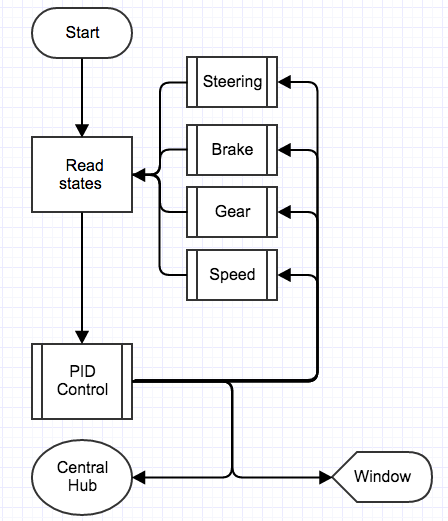
\includegraphics[width=0.6\textwidth]{3-ConceptDesign/autoflowchart.png}
\centering
\caption{Platform automation flow chart} 
\figlabel{autoflowchart}
\end{figure}

 \Figref{autocode} shows that the functions have different processes implemented under each one, with an additional function called emergency stop to be included for safety purposes. This emergency stop function will interrupt all processes if the operator deems it necessary. The specific process under each main function is the "get" and "set" processes. The "get" process is to read the current state of the actuator or servo motor, and the "set" process is to save that current state and expected values in order to calculate the relevant error. There will be further processes added to automate the platform and integrate the navigation path tracking and turning sections.

\begin{figure}[ht]
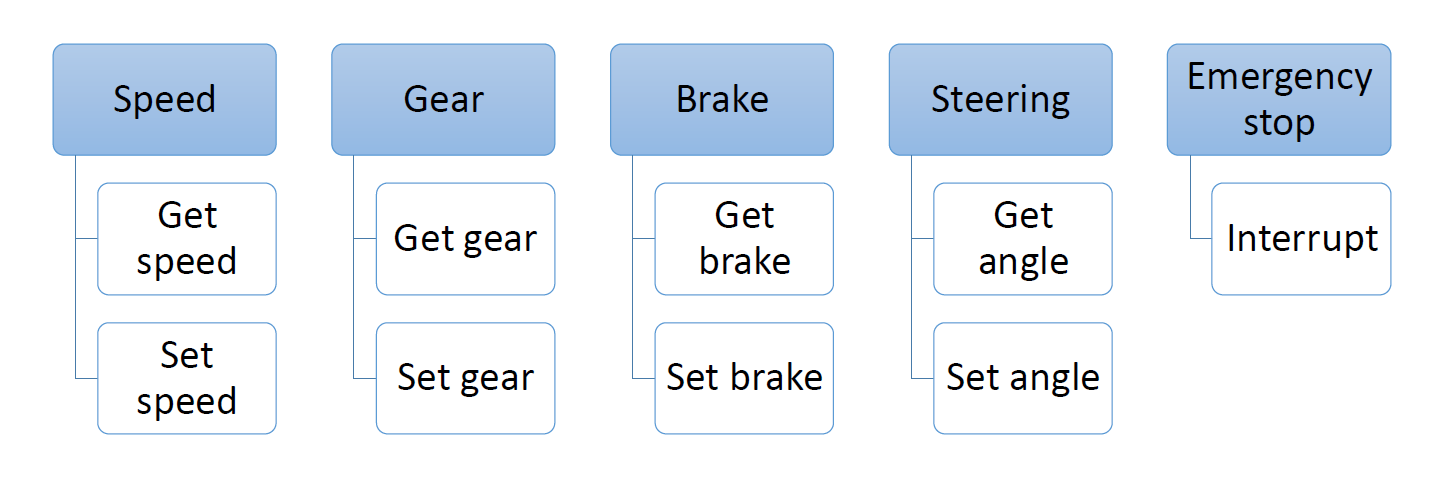
\includegraphics[width=\textwidth]{3-ConceptDesign/autofunct.PNG}
\centering
\caption{Automation code functions} 
\figlabel{autocode}
\end{figure}

\subsection{Path tracking}
\seclabel{pathconcept}
As the platform will be primarily performing two tasks, following a low curvature curve (straight line) and turning a specified angle, the navigation system will define the path using a 'piecewise linear path' discussed in \secref{pathTrackingLitReview}. \Textcite{snider2009} provides an empirical comparison of path following algorithms and is shown in \Figref{trackingComparison}. Tracking methods are ordered by implementation difficulty from least difficult to most difficult. \Textcite{snider2009} goes on to describe recommended applications for each method.  Pure pursuit is ideal in situations for slow driving and/or on discontinuous paths, the Stanley method for smooth highway driving and/or parking manoeuvres, the Kinematic model for smooth parking manoeuvres, and the Dynamic model for highway driving at speed. The most suited to the landmine detection application is slow driving on discontinuous paths and thus Pure Pursuit will be used as the tracking method.
\begin{figure}[ht]
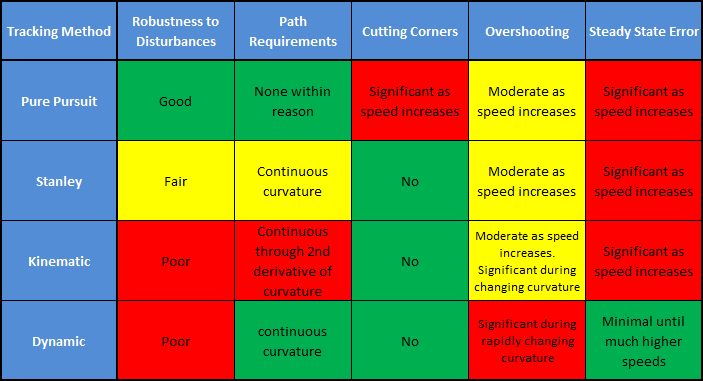
\includegraphics[width = \textwidth]{3-ConceptDesign/pathTrackingSummary2.png}
\centering
\caption[Empirical comparison of path tracking algorithms]{Empirical comparison of path tracking algorithms \parencite{snider2009}} \figlabel{trackingComparison}
\end{figure}

\subsection{Performing turning manoeuvres}
At the end of a swathe the platform will be required to turn a specified angle within a small area defined by the width of the sensing arrays. Alternatively, if the scan history is available to the platform in the form of a map, a larger area may be available to conduct the turn. Due to little or no literature on the unique topic an adaptation of the simplified Ackermann model will be used in conjunction with the Stanley model which excels for parking manoeuvres \parencite{snider2009} to achieve the desired turn.

\subsection{Positioning}
The positioning system is used to determine the location of the quad bike for navigation and to send that data to the user tablet when a mine is detected. Real time positioning in remote locations and accurate to within 0.5m is required from the system. A number of options were looked at when designing the positioning system including Local Positioning Systems (LPS), Global Positioning Systems (GPS), and dead reckoning techniques.

LPS use three or more signalling beacons of known location to determine position through triangulation. They can be highly accurate however, require the signalling beacons to be stationed near the area of interest. Transporting and setting up at least three signalling beacons is a time consuming process and makes for inefficient travelling when numerous areas of interest are present. This was not considered any further as it would require personnel to place beacons in danger zones. 

Similar to LPS, GPS are very accurate. However, due to the distance between receivers and a number of linked effects the positional data is very noisy, providing location reliably within only 4 meters. Better accuracy can be achieved by using correction techniques, such as Real Time Kinematics (RTK), where accuracy increases to sub-centimetre. Similar to LPS, correction methods like RTK require base locations within 15 kilometres of the GPS and can take many seconds to receive a fix, both working against a solution to real time positioning in remote areas.

Dead reckoning techniques calculate the current position by advancing a previous position based on a known speed and heading over some time step. These techniques are highly prone to cumulative error known as drift. A widely used application of dead reckoning is in Inertial Measurement Units (IMU) where accelerometers and gyroscopes are used to determine linear and rotational accelerations and thus have information to update position. This method is able to provide positional data in real time however over longer time periods the accuracy becomes unreliable.

To correct for drift from dead reckoning techniques, GPS aided Inertial Navigation Systems (INS) can be used. Accurate but noisy data from a GPS is constantly fed into an estimation algorithm alongside a smooth, but error accumulating position to correct for the drift. Kalman Filtering is one such technique which is used to combine information from various sensors to provide a much more reliable estimate of position.

\section{Sensor mount}
\seclabel{sensormount}
The sensor mount is required to support the weight of both the GPR and the metal detector as well as be sturdy enough to prevent flexing or warping during operation. The following section describes the basic requirements imposed on the mount.  
\subsection {Requirements} 
The design of the mount must satisfy the performance requirements of each sensor. These include the sensors operating height off the ground and their optimal operating distance from other objects to prevent interference. 

Both the GPR and metal detector must operate horizontally and within close proximity to the ground to ensure no erroneous data.
For minimal ground reflections and interferences, the GPR should operate as close to the ground as possible. Optimal operating conditions for the GPR requires ground contact to trigger the scroll wheel switch. Sensitivity tests to objects above and beside the GPR resulted in little interference. Objects above 50mm had no impact on the data as well as objects 100mm beside it. 

The metal detector is more sensitive to metallic objects above and beside it. A stand-off distance for metallic objects of 500mm is required as well as a vertical stand-off distance of 2 meters. To reduce size, the GPR will be closest to the platform with the metal detector in front, allowing for the required stand-off distance.  
\subsection {Material selection}  
Material selection is largely dependent on the sensor requirements as well as taking into consideration its ease of sourcing, working and repairing. Non metal structures are required due to the metal detector therefore, possible material choices include PVC piping, carbon fibre, wood and fibreglass. \Tabref{sensorMountMaterials} represents decision matrix used to determine the material for the mount.

\begin{table}[ht]
\centering
\caption{Sensor mount material selection matrix}
\tablabel{sensorMountMaterials}
\begin{tabular}{r *4c}
    \multicolumn{1}{r}{}  & \mcrot{1}{l}{45}{\textbf{PVC}} & \mcrot{1}{l}{45}{\textbf{Carbon Fibre}} & \mcrot{1}{l}{45}{\textbf{Wood}} & \mcrot{1}{l}{45}{\textbf{Fibreglass}}\\ \toprule 
    Cost & 10 & 1 & 10 & 3 \\ 
    Ease of manufacture & 10 & 1 & 5 & 3 \\ 
    Ease of repair & 10 & 4 & 8 & 5 \\ 
    Ease to source & 10 & 2 & 10 & 6 \\ 
    Time to build & 10 & 1 & 8 & 10 \\ 
    Strength & 5 & 10 & 6 & 7 \\ \midrule
    \textbf{Total} & 92\% & 32\% & 78\% & 57\% \\ \bottomrule
\end{tabular}
\end{table}

PVC scored the highest due to its low cost, ease to modify and ease of assembly. However, it is not the strongest material and could flex during operation depending on the length.
Carbon fibre is the strongest material but the cost and hardships associated with it resulted in the lowest score. Wood is the second highest but the joining of sections without nails would result in weaker joins. Fibreglass scored in the middle primarily due to the cost and difficulties to manufacture. 
PVC will be used for the primary arm of the supporting bracket holding the metal detector. As strength has been identified as an issue from the selection matrix, future discussions with workshop staff as to the ability to source the required thicknesses to meet the strength criteria, or for the manufacturability of bracing and reinforcement for PVC parts.

%\textcolor{red}{havnt explicitly stated what material we will be using. obviously PVC but then need to offer a solution to the strength issue that comes with PVC. also would it be possible to have metal supporting the gpr then pvc coming off of that to help with the strength issue} 
%% ^^ harry if you want to extend this disucssion still then feel free. but until then i've removed the comment just to clean everything up

\subsection{Initial designs}
Basic design for the sensor mount can be realised with the sensor requirements. Using the DSTG Quad bike as the chosen platform, preliminary designs can be sketched. Considerations for both front and rear mounted sensor arrays were considered. Design 1, 2 and 3 trial different mounting techniques and frame designs.



\subsubsection{Design 1}
Design one is represented in \Figref{design1} and is a rear mounted frame. This mount assumes that the quad bike will be more manoeuvrable when steered from the rear, requiring the direction of travel to be in reverse. Thus, the frame mounting on the back is necessary. 
 \begin{figure}[ht]
 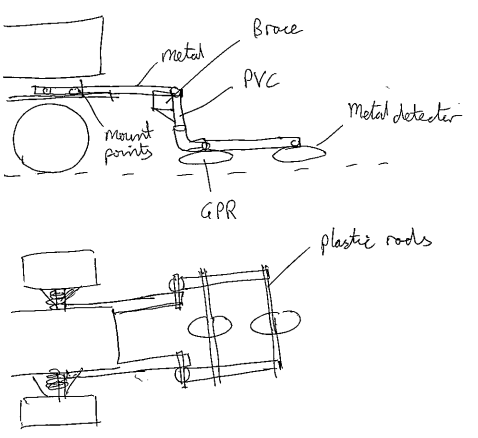
\includegraphics[width=.5\textwidth]{3-ConceptDesign/Rear_Mount.png}
 \centering
 \caption{Rear frame mount concept design}
 \figlabel{design1}
 \end{figure}

\subsubsection{Design 2}
Design 2 represents a front mounted frame assuming that the quad bike is driven in a standard configuration as shown in \Figref{design2}. The GPR is placed in close proximity to the body with the metal detector attached further in front. This design appears to be the smallest and uses the least amount of material.
\begin{figure}[ht]
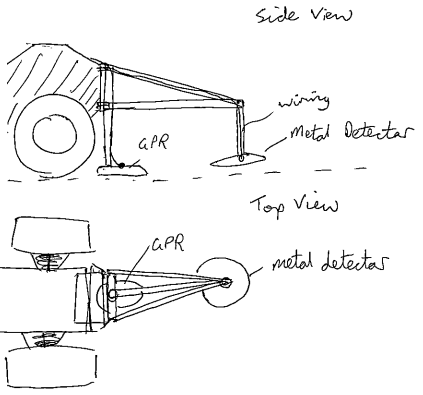
\includegraphics[width=0.5\textwidth]{3-ConceptDesign/front_frame_design_triangle.png}
\centering
\caption{Front frame mount concept design}
\figlabel{design2}
\end{figure}

\subsubsection{Design 3}
Design 3 incorporates a staggered design with the metal detector and GPR placed further in front of the platform as shown in \Figref{design3}. This larger stand off distance would allow for less violent stops as the allowable stopping distance would be increased. However, the required material and weight would be greater potentially requiring greater reinforcements to mitigate flexing and warping. These reinforcements could be from the use of fibreglass coating over the PVC piping.
\begin{figure}[ht]
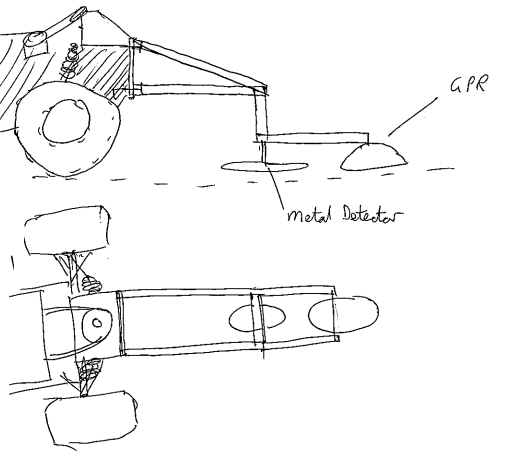
\includegraphics[width=0.5\textwidth]{3-ConceptDesign/front_mount_staggered.png}
\centering
\caption{Front frame mount concept design}
\figlabel{design3}
\end{figure}\\

The sensor mount will be made from a combination of PVC and fibreglass. The fibreglass will be supporting sections to prevent flexing and warping. As exact dimensions and platform performance characteristics are unknown, specific mounting orientation and size cannot be decided upon until the platform is delivered. Once the Platform has been delivered for the project, specific and more detailed designs can be created

\section{Subsystem integration}

\seclabel{conceptprojectdesign}

\subsection{Electronics}
Requirements for the electronics subsystems can be inferred from the project aims. As a major component of the project would be attempting advanced signal processing methods in real time, significant processing capabilities will be required on the mobile platform. In addition to this, the signal processing must be capable of running simultaneously with a number of other platform software systems, such as vehicle control and telemetry. To achieve this without requiring multiple discrete hardware components (which would require communications input/output (I/O) interfaces to share data), a single hardware system capable of executing multiple threads simultaneously and asynchronously is required on the vehicle. The hardware system executing the signal processing software must also be capable of reading sensory input from USB devices, as this is the communications format available on the GPR units provided by the DTSG. 
\nomenclature[A]{I/O}{Input/Output}% 

A second major component of the project is the automation of the remote vehicle, requiring software control over a series of actuators and sensors. To provide the greatest fidelity of control over the vehicle the electronics hardware used to interface with the actuators and sensors must be capable of reading and writing to low-level I/O devices quickly and with minimal latency or overhead. To achieve this, the ability to create hardware interrupts are desirable, which would allow the software to process incoming sensory data as soon as it is received. The software for the parsing and decoding of raw input signals to generate usable information is not expected to be complicated, as so the hardware will not need to be particularly advanced or have capacity for high speed processing.

\begin{itemize}
\item \textbf{Bespoke Electronics}\\
Bespoke electronic equipment has the capacity to allow incredibly fast access to I/O devices through the use of task-specific commercial off-the-shelf (COTS) chips. However, the time consumption and expense of planning an entirely hardware-driven control system for anything more than trivial data handling is inappropriate for this project. The inability to prototype as with software means that the ability to test and then revisit a solution is not possible, and a hardware/purely electronics driven system is not capable of general purpose processing. Therefore, this is not a realistic option for achieving the project aims.
\nomenclature[A]{COTS}{Commercial off-the-shelf}% 
\item \textbf{Microcontrollers}\\
Microcontrollers have become the de facto standard for small to medium software-based projects which require access to physical sensors and actuators, due to their readily available access to low level I/O. Microcontrollers supporting common languages such as C++ and Java allow easy development and rapid prototyping, though the inability to easily connect debugging equipment or generate test output slows the development process. Microcontrollers are inexpensive and provide high I/O availability but at the cost of limited processing power. The low-level nature of microcontrollers means that desirable features like hardware interrupts are exposed to and accessible by developers. 
\item \textbf{Desktop computing equipment/Laptop} \\
Conventional desktop computing equipment is the fastest general purpose computing hardware that will be available to the project. In addition to having the greatest computing power, it has the highest ability to support prototyping and allows for rapid software development with readily accessible software generation and debugging tools. The drawback of this higher-level computing platform is the reduced accessibility of low-level I/O devices, and the amount of computing overhead caused by operating system processes. Operations that require fast I/O access may be hampered by the inability to ensure thread availability, and so for robust operation this may require buffering to a secondary, lower level device.
\end{itemize}

None of the individual items presented allow for the full range of requirements of this project. As a result, the general concept for the hardware arrangement to execute the software systems is shown below in \Figref{hardwareLayout}.
% is this figure text fucking big enough maziar??
\begin{figure}[ht]
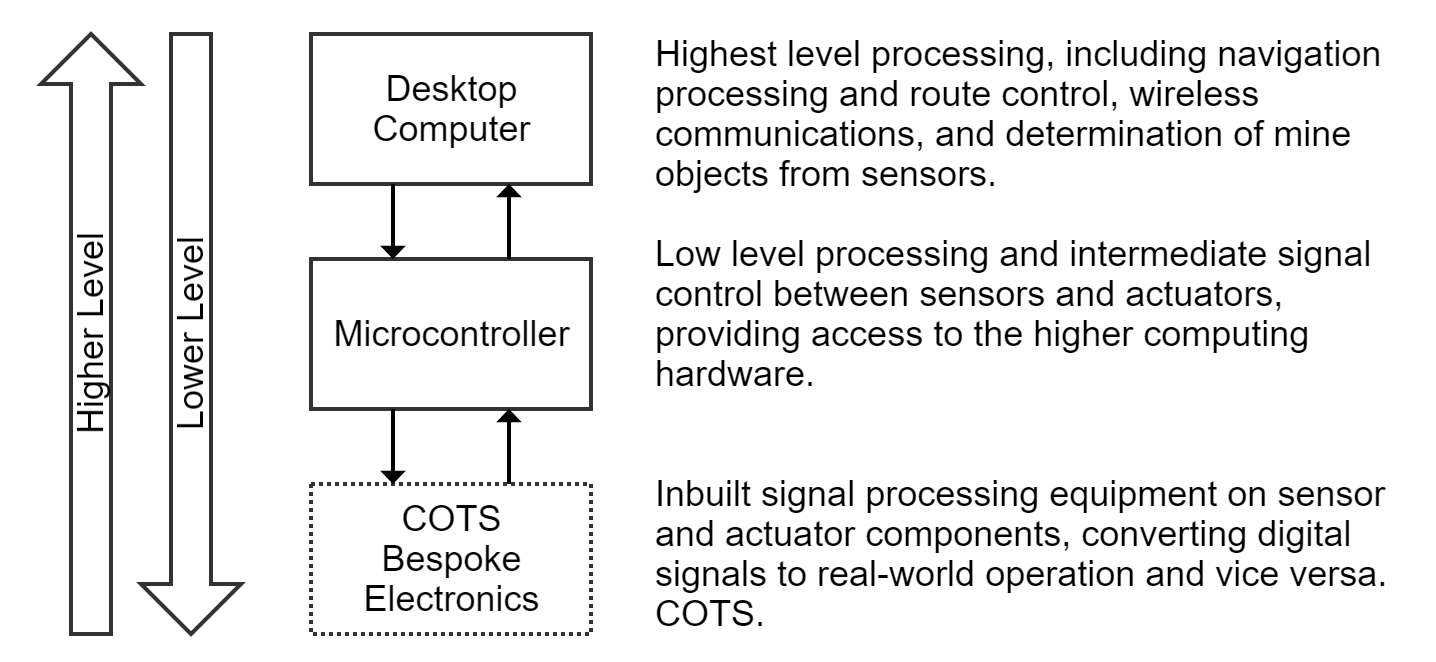
\includegraphics[width = \textwidth]{3-ConceptDesign/electronics.png}
\centering
\caption{Conceptual hardware layout} \figlabel{hardwareLayout}
\end{figure}

Under this system, the project will use standard desktop computing equipment for the bulk of the software, to make use of its superior processing power and the rapid development it allows. This device will be the data handler and processor, and act as the 'central' software location for the project. Sensors and actuators that require low level I/O access will be connected to a secondary microcontroller, which will act independently to buffer inputs and outputs of the system, which can then be communicated to the primary computer over a serial communications connection. The project will not aim to develop any custom electronics boards and handle all signal amplification or processing in software.

\begin{figure}[ht]
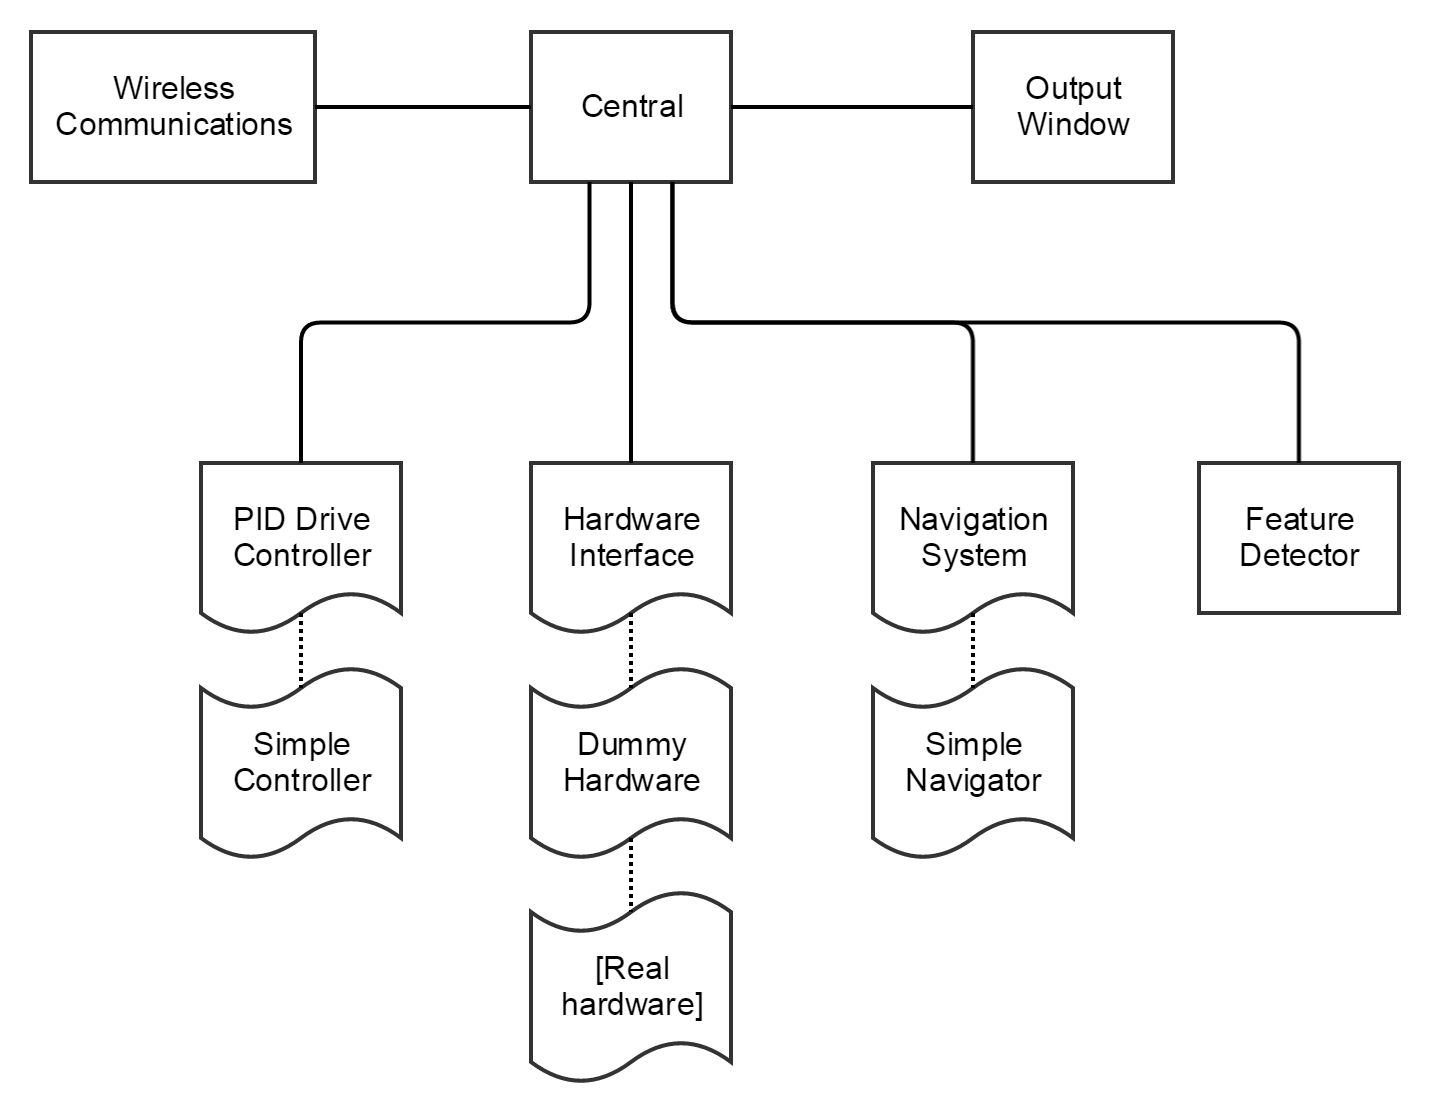
\includegraphics[width=\textwidth]{3-ConceptDesign/fyp_structure.png}
\centering
\caption{Integration of automation, navigation, sensors and signal processing} 
\figlabel{central}
\end{figure}

\subsection{Software architecture}
The autonomous quad bike will be used as the platform on which the sensor mount and software subsytems will operate. A concept is shown in \Figref{frontConcept} and \Figref{rearConcept}. To achieve the framework for overall automation of the platform the integration of the actuator electronics, navigation, sensors, signal processing and operator device is required. This framework is completed through the Central Hub as shown in \Figref{central} where dotted lines indicate implementations of the interfaces. The Central Hub will combine and read all the relevant processes and transmit the required information to the operator device. This enables all processes to be completed in parallel, satisfying the deliverables as defined in \secref{primary}.

\begin{figure}[ht]
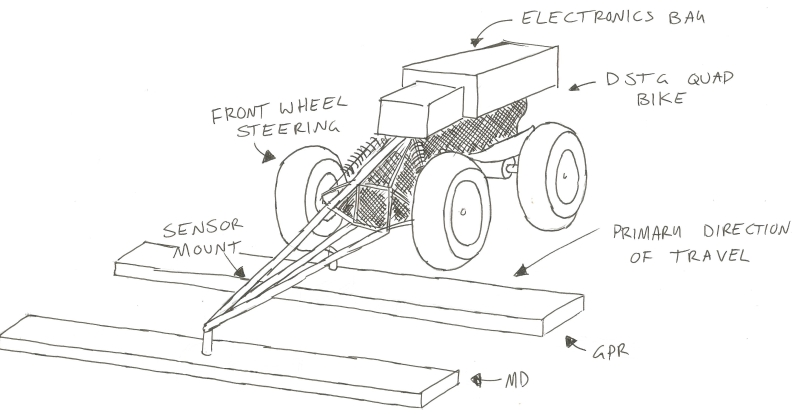
\includegraphics[width = 0.8\textwidth]{3-ConceptDesign/ConceptFront.jpeg}
\centering
\caption{Front wheel drive platform concept design} \figlabel{frontConcept}
\end{figure}
\begin{figure}[ht]
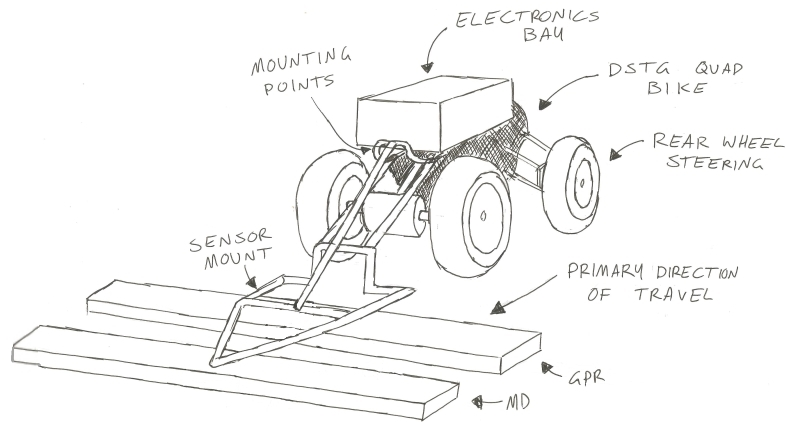
\includegraphics[width = 0.8\textwidth]{3-ConceptDesign/ConceptRear.jpeg}
\centering
\caption{Rear wheel drive platform concept design} \figlabel{rearConcept}
\end{figure}

The DSTG quad bike provides a basis to apply the completed concept designs and build upon them in order to have detailed designs for the automation and signal processing. 

\subsection{Communications}

\end{document}